\subsection{Area 1 – Aule}
\begin{figure}[H]
\centering
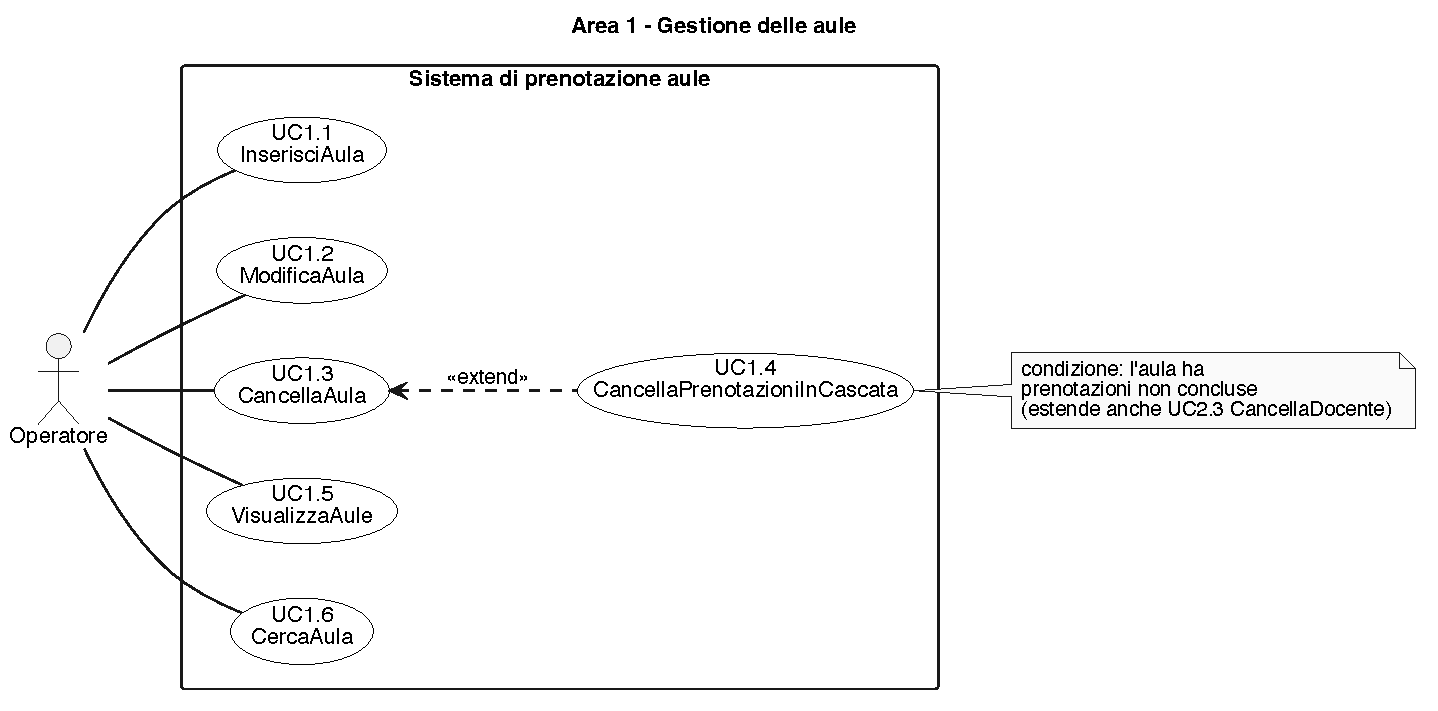
\includegraphics[width=\textwidth,height=0.8\textheight,keepaspectratio]{diagrammi/uc-area1-aule}
\caption{Casi d'uso dell'Area 1 – Aule}
\end{figure}

\subsubsection{[UC1.1] InserisciAula}
\noindent Attore: Operatore\\
Requisiti correlati: FI1.1, ED1.1–ED1.4, IU1.1, IU1.2, IU4.6, IU4.7\\
Pre-condizioni: Il sistema mostra la sezione Aule.\\
Post-condizioni: La nuova aula è registrata nell'archivio, l'archivio è salvato su file e l'aula compare nella lista delle aule.\\

\noindent Flusso principale:
\begin{enumerate}
\item L'Operatore sceglie il comando Nuova aula.
\item Il sistema mostra il modulo dell'aula con i campi codice, nome, edificio, piano e capienza vuoti.
\item L'Operatore compila i campi e conferma.
\item Il sistema verifica che i dati rispettino i vincoli ED1.1, ED1.3 ed ED1.4.
\item Il sistema verifica che non esista un'altra aula con lo stesso codice (ED1.2).
\item Il sistema registra l'aula, salva l'archivio, chiude il modulo e mostra la lista aggiornata con un messaggio di esito.
\end{enumerate}
\noindent Flussi alternativi:
\begin{itemize}
\item \textbf{3a.} L'Operatore annulla: si applica FC1.
\item \textbf{4a.} Uno o più dati non sono validi (es. campo vuoto, capienza non intera o non positiva):
\begin{itemize}
\item 4a.1 Il sistema indica ogni campo errato e il vincolo da rispettare (IU4.6);
\item 4a.2 si riprende dal passo 3.
\end{itemize}
\item \textbf{5a.} Esiste già un'aula con lo stesso codice:
\begin{itemize}
\item 5a.1 Il sistema segnala che il codice è già in uso;
\item 5a.2 si riprende dal passo 3.
\end{itemize}
\item \textbf{6a.} Il salvataggio non riesce: si applica FC2.
\end{itemize}

\subsubsection{[UC1.2] ModificaAula}
\noindent Attore: Operatore\\
Requisiti correlati: FI1.2, ED1.1–ED1.4, IU1.1, IU1.2, IU4.6, IU4.7\\
Pre-condizioni: Il sistema mostra la sezione Aule e nell'archivio è registrata almeno un'aula.\\
Post-condizioni: I dati dell'aula sono aggiornati nell'archivio, l'archivio è salvato su file e la lista mostra i nuovi valori. Codice e prenotazioni dell'aula non cambiano.\\

\noindent Flusso principale:
\begin{enumerate}
\item L'Operatore seleziona un'aula nella lista (o tra i risultati di una ricerca) e sceglie il comando Modifica.
\item Il sistema mostra il modulo dell'aula con i dati attuali; il codice è visibile ma non modificabile.
\item L'Operatore modifica uno o più campi tra nome, edificio, piano e capienza e conferma.
\item Il sistema verifica che i dati rispettino i vincoli ED1.1, ED1.3 ed ED1.4.
\item Il sistema aggiorna l'aula, salva l'archivio, chiude il modulo e mostra la lista aggiornata con un messaggio di esito.
\end{enumerate}
\noindent Flussi alternativi:
\begin{itemize}
\item \textbf{1a.} L'Operatore sceglie Modifica senza aver selezionato un'aula:
\begin{itemize}
\item 1a.1 Il sistema chiede di selezionare un'aula;
\item 1a.2 si riprende dal passo 1.
\end{itemize}
\item \textbf{3a.} L'Operatore annulla: si applica FC1.
\item \textbf{4a.} Uno o più dati non sono validi:
\begin{itemize}
\item 4a.1 Il sistema indica ogni campo errato e il vincolo da rispettare;
\item 4a.2 si riprende dal passo 3.
\end{itemize}
\item \textbf{5a.} Il salvataggio non riesce: si applica FC2.
\end{itemize}

\subsubsection{[UC1.3] CancellaAula}
\noindent Attore: Operatore\\
Requisiti correlati: FI1.3, FI1.4, IU4.3, IU4.7, NF7\\
Pre-condizioni: Il sistema mostra la sezione Aule e nell'archivio è registrata almeno un'aula.\\
Post-condizioni: L'aula e le sue prenotazioni concluse sono rimosse dall'archivio, l'archivio è salvato su file e l'aula non compare più nella lista.\\
Punto di estensione: Passo 2: l'aula ha prenotazioni non concluse $\rightarrow$ UC1.4 CancellaPrenotazioniInCascata.\\

\noindent Flusso principale:
\begin{enumerate}
\item L'Operatore seleziona un'aula nella lista e sceglie il comando Cancella.
\item Il sistema verifica che l'aula non abbia prenotazioni non concluse.
\item Il sistema chiede conferma mostrando i dati dell'aula (IU4.3).
\item L'Operatore conferma.
\item Il sistema rimuove l'aula e le sue eventuali prenotazioni concluse, salva l'archivio e mostra la lista aggiornata con un messaggio di esito.
\end{enumerate}
\noindent Flussi alternativi:
\begin{itemize}
\item \textbf{1a.} L'Operatore sceglie Cancella senza aver selezionato un'aula:
\begin{itemize}
\item 1a.1 Il sistema chiede di selezionare un'aula;
\item 1a.2 si riprende dal passo 1.
\end{itemize}
\item \textbf{2a.} L'aula ha almeno una prenotazione non conclusa:
\begin{itemize}
\item 2a.1 si esegue UC1.4 CancellaPrenotazioniInCascata e il caso d'uso termina.
\end{itemize}
\item \textbf{4a.} L'Operatore annulla: si applica FC1.
\item \textbf{5a.} Il salvataggio non riesce: si applica FC2.
\end{itemize}

